\documentclass[letterpaper,10pt,conference]{ieeeconf}

\IEEEoverridecommandlockouts
\overrideIEEEmargins

\usepackage{graphicx}
\usepackage{amsmath,amssymb}
\usepackage{booktabs}
\usepackage{microtype}
\usepackage{xcolor}
\usepackage{url}
\usepackage{balance}

\title{\LARGE \bf
From Future Danger to Communication Value:\\
Risk-Aware Visual Communication for Robot Navigation}

\author{Shirong Zuo$^{1}$%
\thanks{$^{1}$Shirong Zuo is with the School of Artificial Intelligence,
Xidian University, Xi'an, China.}}

\newcommand{\send}{\mathsf{send}}
\newcommand{\hold}{\mathsf{hold}}

\begin{document}
\maketitle
\thispagestyle{empty}
\pagestyle{empty}

\begin{abstract}
A bandwidth-limited robot cannot communicate every camera update, yet an early
warning of danger does not identify when a packet is worth spending. We study
this distinction through a causal Webots pipeline that combines deterministic
ego-motion rollout, decision-level visual Safety Value, and an interpretable
feasibility-deterioration precursor. In an independently sealed evaluation of
240 physical configurations, future-motion-conditioned danger raises 2-s
AUPRC from 0.9063 to 0.9937 (difference 0.0874, 95\% CI
[0.0772, 0.0985]). Without refitting, the precursor anticipates 16 of 19
Safety-Value onsets across four new physical families with 0.576-s median lead
while active for 1.465\% of time. We then compare SEND NOW with preserving the
same packet using identical-prefix, exactly 72,000-byte branches. Thirty direct
opportunities are helpful in 13 cases, harmful in 7, and neutral in 10. After
repairing the target to adjacent opportunities, 45 comparisons contain
11/15/19 helpful/harmful/neutral cases, but the best leave-family-out causal
model reaches only 0.628 helpful AUPRC and fails its frozen selection gate.
Thus future danger, decision relevance, and immediate transmission utility are
empirically distinct; no safer scheduler is claimed.
\end{abstract}

\section{Introduction}

Visual observations support obstacle avoidance, but transmitting them at the
camera rate is often incompatible with constrained or intermittent links. The
central scheduling question is therefore not merely whether an image contains
important content; it is which update deserves one of the remaining
communication opportunities. Task-oriented image coding and collaborative
perception address rate--task trade-offs \cite{liu2022task,hu2022where2comm},
while learned communication systems decide where, when, or with whom agents
exchange features \cite{liu2020when2com,wang2020v2vnet}. For closed-loop
navigation, however, ``dangerous,'' ``decision-relevant,'' and ``useful to send
now'' need not describe the same instant.

Consider a robot whose present motion makes a later obstacle encounter
predictable. Future risk may rise before the obstacle produces a materially new
camera observation. Later, a fresh frame may change the receiver's feasible
motion set, but sending it immediately can still be suboptimal if only a few
packets remain and a more consequential transition follows. This creates a
temporal hierarchy: future danger is an early physical forecast; decision value
asks whether fresh visual information changes safe planning; transmission
utility asks whether consuming a packet now improves the eventual closed loop.

We investigate this hierarchy through a sequence of frozen, causal experiments
(Fig.~\ref{fig:overview}). The sender and receiver use only current or past
decoded visual information and robot-local state. Physical contact, true
clearance, and future simulator states remain evaluator-only. Real serialized
packet bytes are counted, and competing closed-loop policies receive the same
episode budget.

\begin{figure*}[t]
  \centering
  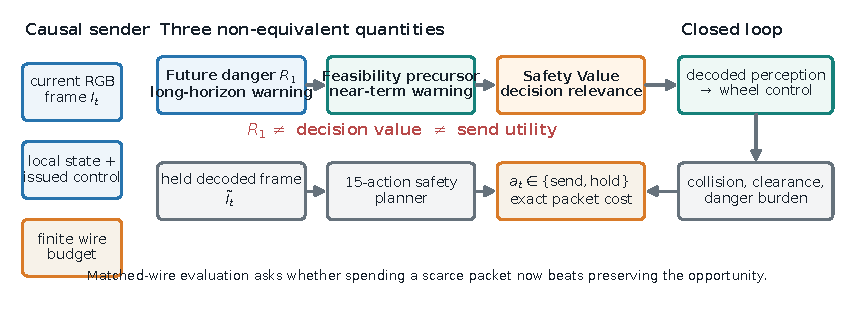
\includegraphics[width=.985\textwidth]{figures/fig1_system_overview.pdf}
  \caption{Causal study design. Predicted danger can precede a deterioration of
  the receiver's feasible action set; Safety Value confirms that a fresh frame
  changes the safety decision. Neither signal alone establishes that spending a
  finite packet immediately is better than holding it for a later observation.}
  \label{fig:overview}
\end{figure*}

This paper makes exactly three contributions:
\begin{enumerate}
\item A causal future-danger formulation based on deterministic ego-motion
rollout, independently confirmed on a sealed set of 240 physical
configurations.
\item A decision-space definition of visual Safety Value and a frozen,
cross-scenario feasibility precursor that anticipates 16/19 onsets with
0.576-s median lead while active only 1.465\% of the time.
\item An exact matched-wire counterfactual study that directly measures
helpful, harmful, and neutral packet opportunities, exposes narrow utility
windows, and reports a bounded negative result when causal utility models fail
cross-family selection gates.
\end{enumerate}

\section{Related Work}

\subsection{Task-Oriented Robotic Communication}
Task-oriented image communication jointly considers rate, reconstruction, and
downstream distortion rather than pixel fidelity alone \cite{liu2022task}.
TAGIC similarly uses task context to guide image communication for simulated
teleoperation \cite{diao2024tagic}. Multi-agent perception methods learn when
to establish communication groups \cite{liu2020when2com}, transmit spatially
sparse high-confidence features \cite{hu2022where2comm}, or exchange compressed
features for joint perception and forecasting \cite{wang2020v2vnet}. These
systems demonstrate that task relevance can reduce communication, but their
primary endpoints are reconstruction, perception, or forecasting. Our endpoint
is matched-cost closed-loop navigation, and our variable of interest is the
temporal marginal value of one visual packet.

\subsection{Predictive Risk and Information Timing}
Predictive attention can place visual processing on regions likely to affect
future control and unsafe-condition detection \cite{lee2020perceptual}.
Risk-aware spatio-temporal corridors likewise convert predicted environmental
evolution into constraints for motion planning \cite{chen2023rast}. Our work
does not claim to introduce task-oriented communication, predictive attention,
or risk-aware planning. It instead tests whether future physical danger,
receiver-side decision relevance, and immediate packet utility coincide. The
matched-wire intervention reveals that they do not.

\section{Problem Formulation}

At control step $t$, the sender observes robot-local state $s_t$, the issued
wheel command $u_t$, and camera frame $I_t$. The receiver controls from the most
recently decoded frame $\tilde I_t=I_{\ell(t)}$, where $\ell(t)\leq t$ is the
last send time. A causal policy has information
\begin{equation}
\mathcal I_t=\{s_\tau,u_\tau,I_\tau,a_\tau:\tau\leq t\}
\cup\{\tilde I_t,b_t\},
\end{equation}
where $b_t$ is remaining wire budget and
$a_t\in\{\send,\hold\}$. It cannot access future frames, future physical
states, contact, or evaluator geometry.

Let $\Pi(I,s)$ be a frozen safety-first local planner. We distinguish three
quantities. Future danger $R_{1,t}$ scores whether the current motion is headed
toward low clearance. Decision value $V_t$ indicates whether planning with
$I_t$ rather than $\tilde I_t$ produces a material safety transition. Immediate
transmission utility is the counterfactual closed-loop benefit of choosing
$\send$ instead of $\hold$ while preserving future budget consequences. The
last quantity is not assumed equal to either $R_{1,t}$ or $V_t$.

If a serialized packet costs $c=24{,}000$ bytes including codec and protocol
overhead, all primary Q6 policies obey
\begin{equation}
\sum_t c\,\mathbb I[a_t=\send]=72{,}000~\text{bytes/episode}.
\label{eq:budget}
\end{equation}
The receiver decodes each transmitted packet and holds that reconstruction
between sends. Thus equal nominal rates are insufficient: Eq.~\eqref{eq:budget}
is checked from actual wire records.

\section{Method}

\subsection{Predictive Ego Danger}
The motion predictor is deterministic differential-drive kinematics, not a
learned model. For wheel rates $(\omega_L,\omega_R)$, wheel radius $r_w$, and
axle length $L$, the twist is
\begin{equation}
v=\tfrac{r_w}{2}(\omega_R+\omega_L),\qquad
\Omega=\tfrac{r_w}{L}(\omega_R-\omega_L),
\end{equation}
and is integrated exactly as a constant twist over 32-ms increments. The
state-only rollout holds measured $(v,\Omega)$ constant. The
command-conditioned rollout instead converts the issued wheel-command schedule
to a piecewise-constant twist. Their all-stable ADEs at 0.5/2.0 s are
$1.20561\!\times\!10^{-4}/7.15992\!\times\!10^{-4}$ m (state-only) and
$6.398\!\times\!10^{-6}/1.3655\!\times\!10^{-5}$ m
(command-conditioned).

For each polyline $\Gamma_{k,t}$ and currently represented obstacle set
$\mathcal O_t$, define physical-footprint clearance
\begin{equation}
d_{k,t}=\min_{p\in\Gamma_{k,t},\,o\in\mathcal O_t}
\operatorname{dist}(p,o)-r_b, \qquad R_{k,t}=-d_{k,t},
\label{eq:risk}
\end{equation}
with body radius $r_b=0.037$ m. $R_0$ uses the current center point;
$R_1$ uses the state-only 2-s rollout and is the primary downstream risk
signal; $R_2$ uses the command schedule and is secondary/mechanistic. This
naming follows the frozen M9 implementation.

\subsection{Decision-Level Safety Value and Precursor}
The receiver evaluates 15 local actions: three forward speeds crossed with
five angular rates. Each 1.5-s trajectory has conservative minimum clearance
$m_{i,t}$ from decoded visual obstacle estimates, including range uncertainty.
It is hard-feasible at $m_{i,t}\geq h=0.025$ m and preferred-safe at
$m_{i,t}\geq p=0.075$ m. Selection prioritizes preferred-safe moving actions,
then hard-safe maximum-margin actions, and finally stop.

Safety Value compares the held-image plan with a shadow plan from the current
causal image. It triggers if any frozen condition holds: (i) selected safety
class deteriorates; (ii) a nonempty moving-safe set collapses; (iii) the held
action changes and is no longer hard-feasible; or (iv) at least one third of
held-safe actions disappear and the held action's matched margin falls by at
least 0.01 m (transition from infinite to finite margin also counts as a large
drop). A Q5 onset must additionally occur after step 7, before contact, and
retain at least two current safe alternatives. This is decision-level value,
not an arbitrary path change or pixel difference.

The precursor uses the exact soft feasibility mass of the current plan. With
$N=15$, $s=p-h=0.05$ m, and finite replacement
$\bar m_{i,t}=m_{i,t}$ if finite or $p+20s$ otherwise,
\begin{align}
z_{i,t}&=\operatorname{clip}\!\left(
\frac{\bar m_{i,t}-h}{s},-60,60\right),\\
\Phi_t&=\frac{1}{N}\sum_{i=1}^{N}\frac{1}{1+e^{-z_{i,t}}}\in[0,1].
\label{eq:softmass}
\end{align}
If every margin is non-finite, the implementation sets $\Phi_t=1$.
For the eight past-through-current samples $y_j=\Phi_{t-7+j}$ at
$\tau_j=0.032j$ s, the causal OLS slope is
\begin{equation}
\beta_t=\frac{\sum_{j=0}^{7}(\tau_j-\bar\tau)(y_j-\bar y)}
{\sum_{j=0}^{7}(\tau_j-\bar\tau)^2}.
\end{equation}
No future sample enters $\beta_t$. With the exact frozen constants
\begin{align}
\phi^*&=0.6543448254639964,\nonumber\\
\beta^*&=-0.11876628431105299~\mathrm{s}^{-1},\nonumber
\end{align}
the precursor is
\begin{equation}
P_t=\mathbb I[\Phi_t\leq\phi^*\ \land\ \beta_t<\beta^*].
\label{eq:precursor}
\end{equation}

\subsection{Causal Matched-Budget Probe}
The closed-loop probe sends three 24-kB decoded-image packets. $U_0$ uses the
fixed schedule $\{0,109,218\}$. $A_0$ uses current clearance risk $R_0$ in the
same causal scheduling stack. The final precursor policy uses $R_1$, requires
two consecutive $P_t=1$ samples, and spends its middle packet when that
persistent opportunity is available; otherwise it falls back at step 217. A
startup packet at step 0 and protected reserve at step 218 are fixed. A
precursor opportunity remains valid for 25 steps. Codec, decoded perception,
planner, controller, physical cell, and total bytes are shared. This policy is
an intervention probe, not a selected final method.

\section{Experimental Protocol}

Experiments use Webots R2025a and an e-puck. All steps log sender signals,
serialized packets, decoded receiver image, planner state, wheel control,
bilateral contact, and physical clearance. Online modules do not receive true
obstacle geometry. Physical labels use the frozen 0.037-m footprint and a
near-danger boundary of 0.013 m.

\textbf{Future danger.} M9-B is an independent sealed replication with 240
distinct physical configurations: 70 collision, 70 buffered-near, and 100
safe. Its primary endpoint is family-macro 2-s danger AUPRC for $R_1-R_0$,
with a 10,000-replicate paired, episode-stratified bootstrap. $R_2-R_1$ is
descriptive only.

\textbf{Precursor.} Q5 attempts eight new physical families without using
precursor outputs in scenario construction. Four produce accepted Safety-Value
support: staggered slalom, three-stage weave, opposed gate contraction, and
reverse diagonal chicane. The frozen rule is applied once to 19 accepted onsets
and 53 event-free episodes. Coverage requires activity strictly before onset;
lead is measured from the first active sample in the bounded look-back window.

\textbf{Closed loop.} Q6 comprises 140 new Webots executions over three
bounded scheduler generations. The final generation is compared on 20 paired
cells (five per positive family) against sealed $U_0$ and $A_0$ controls.
Primary diagnostics are danger steps and minimum physical clearance. Packet
reconciliation and receiver mirroring must pass for each run. No method is
selected from Q6; no confirmatory scheduler study or hardware experiment is
claimed.

\textbf{Packet opportunity value.} Q6.5 adds five physical families and two
development generations. Each paired branch has an identical prefix, three
real 24,000-byte packets, and a protected final reserve. Safety utility is
lexicographic: collision, then a three-step difference at the frozen 0.12-m
danger boundary, then a 1-mm minimum-clearance difference. Generation 2 uses
60 fixed-schedule runs to compare adjacent opportunities at steps 80, 109,
144, and 217. Models use leave-one-family-out folds; scenario identity and
evaluator outcomes are forbidden inputs.

\section{Results}

\begin{figure*}[t]
  \centering
  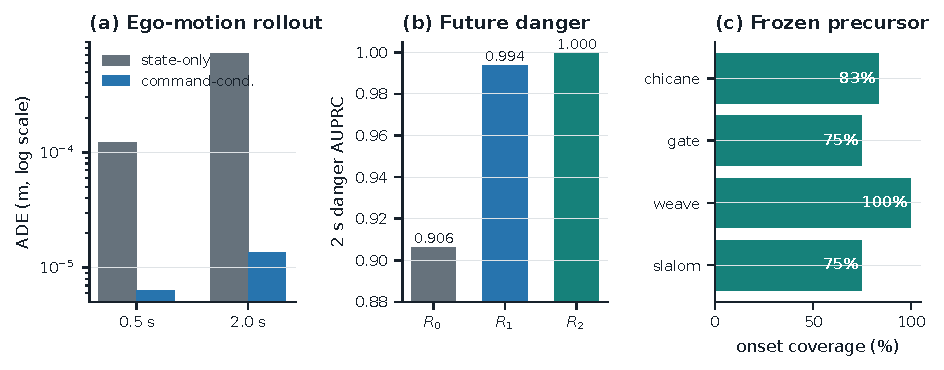
\includegraphics[width=.985\textwidth]{figures/fig2_evidence_chain.pdf}
  \caption{Evidence chain. (a) Command conditioning improves deterministic
  ego-motion rollout accuracy. (b) In sealed M9-B, future-motion risk $R_1$
  improves 2-s danger discrimination over current-state $R_0$; $R_2$ is
  secondary. (c) The unchanged precursor transfers to four new
  Safety-Value-positive families.}
  \label{fig:evidence}
\end{figure*}

\subsection{Future Motion Predicts Physical Danger}
M9-B retains all 240 configurations with zero exclusions and passes every
support gate. At 2 s, family-macro AUPRC is 0.906311 for $R_0$, 0.993730 for
$R_1$, and 0.999778 for secondary $R_2$. The preregistered primary difference
$R_1-R_0$ is 0.087419 with 95\% CI [0.077181, 0.098534]. Continuous-clearance
MAE falls from 0.021085 m ($R_0$) to 0.003618 m ($R_1$) and 0.001829 m
($R_2$). Thus future rollout is a reliable danger signal, while the additional
command schedule explains a smaller secondary gain (Fig.~\ref{fig:evidence}).

Earlier closed-loop diagnostics show why this does not directly solve timing.
Across six supported traces, the $R_1$ trigger leads the 25\%-cumulative visual,
perception, and control-change times by median 2.976, 2.912, and 3.760 s,
respectively, and precedes peak control sensitivity by 4.544 s. Risk lead is
therefore not communication-value lead.

\subsection{Decision Relevance Can Be Anticipated}
Q5 yields 19 accepted onsets in four new positive families. The unchanged
precursor covers 16/19 (84.21\%); per-family coverage is 75\%, 100\%, 75\%,
and 83.3\%. Covered-event lead has mean 0.648 s, median 0.576 s, interquartile
range 0.432--0.776 s, and range 0.352--1.344 s. The indicator is active in
320/21,840 samples (1.465\%). It activates in 11/53 event-free episodes
(20.75\%). Median available opportunity is 0.224 s, and all 16 covered onsets
have at least two consecutive active samples.

The online composite takes 0.126 ms on average, 0.220 ms at the 95th
percentile, and 0.578 ms maximum, with 0/1000 misses of the 32-ms control
deadline. These results qualify $P_t$ as an efficient cross-scenario precursor
to decision relevance, not as evidence of packet utility.

\begin{table}[t]
\centering
\caption{Causal evidence and claim boundary.}
\label{tab:results}
\footnotesize
\setlength{\tabcolsep}{3.2pt}
\begin{tabular}{@{}p{.15\columnwidth}p{.42\columnwidth}p{.32\columnwidth}@{}}
\toprule
Stage & Main result & Supported claim \\
\midrule
M9-B & $R_1-R_0$ AUPRC $=0.0874$, CI $[.0772,.0985]$ & Future motion predicts danger \\
Q5 & 16/19 onsets, 0.576-s median lead, 1.465\% active & Decision relevance is anticipatable \\
Q6 vs $A_0$ & $-40.9$ danger steps, $+19.75$ mm; 9/11/0 improve/tie/adverse & Better than reactive baseline \\
Q6 vs $U_0$ & $-10.3$ danger steps, $-1.24$ mm; 8/4/8 & No consistent strongest-baseline safety gain \\
Q6.5 & 11/15/19 helpful/harmful/neutral; best AUPRC 0.628 & Utility measurable; no predictor selected \\
\bottomrule
\end{tabular}
\end{table}

\subsection{Relevance Does Not Guarantee Send Utility}
All 140 Q6 runs transmit exactly 72,000 wire bytes; reconciliation and receiver
mirroring pass. Relative to $A_0$, the final rule reduces mean danger burden by
40.9 steps and raises minimum clearance by 19.75 mm. Nine cells improve, 11
tie, and none are adverse. Reporting only this comparison would be misleading.

Against the stronger $U_0$, danger burden still falls by 10.3 steps on average,
but minimum clearance falls by 1.24 mm. Outcomes split evenly: 8 improve, 4
tie, and 8 are adverse. Family effects are heterogeneous
(Fig.~\ref{fig:q6}). The staggered-slalom family is materially adverse, adding
26.2 danger steps and losing 14.0 mm clearance, whereas three-stage weave
improves both measures. No collision-count difference is observed.

\begin{figure*}[t]
  \centering
  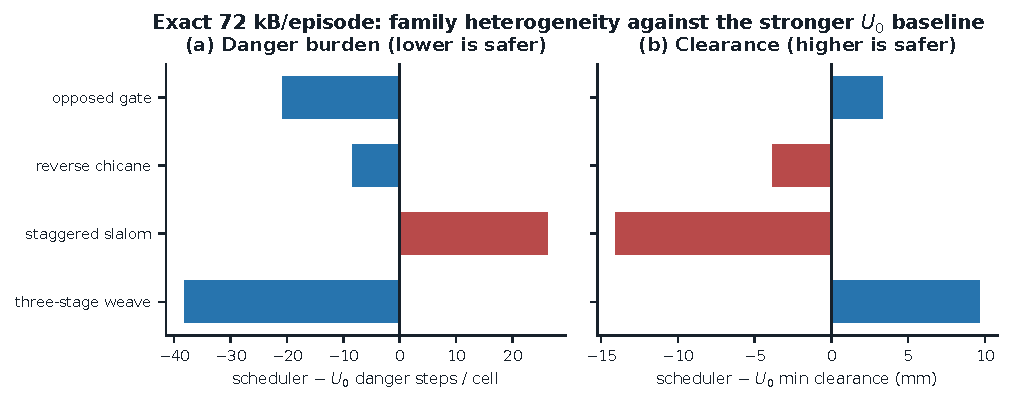
\includegraphics[width=.90\textwidth]{figures/fig3_q6_closed_loop.pdf}
  \caption{Final scheduler effects against the stronger matched-byte $U_0$
  baseline. Blue denotes the safer direction and red the adverse direction.
  Correctly anticipating decision relevance does not yield uniform packet
  utility across physical families.}
  \label{fig:q6}
\end{figure*}

A post-hoc grouped diagnostic tested whether a compact learned precursor could
repair this heterogeneity. Held-family macro AUPRC was only 0.267 for logistic
regression and 0.445 for a tree, with false-warning episode fractions 56.6\%
and 83.0\%, versus 20.8\% for the frozen rule. Neither model was integrated.

\subsection{Packet Utility Is Measurable but Not Safely Predicted}
Q6.5 intervenes on packet timing rather than treating relevance as a proxy.
Thirty matched SEND/HOLD pairs yield 13 helpful, 7 harmful, and 10 neutral
opportunities. A runtime-aligned logistic model reaches 0.911
leave-family-out AUPRC, yet its scheduler is worse than $U_0$: mean danger
increases by 1.73 steps and minimum clearance falls by 1.42 mm. It had learned
SEND versus a step-217 fallback, not SEND versus $U_0$'s step-109 opportunity.

Generation 2 freezes adjacent comparisons before a four-schedule bank. Its 45
opportunities contain 11 helpful, 15 harmful, and 19 neutral labels. Utility is
non-monotonic: in each split-gate cell, steps 80 and 109 collide, step 144
avoids collision, and step 217 collides again. The best binary logistic model
obtains 0.642 AUPRC with 40\% harmful false sends. A preregistered three-class
rule reduces harmful false sends to 20\%, but helpful AUPRC is only 0.628 and
recall 45.5\%. It fails the frozen gate; no method or Q7 study is opened.

\balance
\section{Discussion}

The experiments support a strict hierarchy: future risk $\neq$ decision value
$\neq$ immediate transmission utility.
Future risk is predictable seconds before received-image changes strongly
affect control. Feasible-set deterioration narrows this gap and anticipates
when fresh visual information changes the safety decision. Yet that relevance
is only a necessary condition for useful communication. Under a finite packet
budget, a relevant frame competes with unknown future observations.

This opportunity cost explains the Q6 pattern. $A_0$ reacts late enough that a
decision-aware precursor can improve it. $U_0$, however, preserves a later
observation at a fixed time; in sequential obstacles that later packet can be
more valuable than the first persistent precursor. The staggered-slalom result
is a concrete counterexample to treating $P_t$ as a direct SEND command. The
scientific contribution is therefore not a universally safer scheduler, but an
experimentally grounded decomposition of what such a scheduler must estimate.

Q6.5 makes the remaining target operational: communication action value is the
physical safety difference between adjacent, equal-cost SEND/HOLD branches.
It can be measured reproducibly, but the current causal state does not predict
it safely across held-out families. Risk magnitude or current decision change
alone cannot substitute for unobserved future opportunity structure.

Limitations are substantial. Evidence comes from Webots, one robot model, a
controlled visual detector, and a fixed 15-action planner. The exact thresholds
in Eq.~\eqref{eq:precursor} are system-specific. Q5 is development
qualification, while Q6 and Q6.5 are bounded development interventions rather
than sealed confirmatory scheduler evaluations. Q6.5 reuses its 15 cells for
model development and cross-family replay; it is not independent validation.
No method freeze, Q7, formal scheduler result, or real-robot validation exists.
These boundaries preclude a claim of closed-loop safety improvement.

\section{Conclusion}

We studied when scarce visual updates should be communicated for robot
navigation. A sealed 240-configuration evaluation confirms that future-motion
risk predicts danger, and a frozen feasibility precursor anticipates
decision-relevant visual changes across four new families. Exact matched-wire
closed-loop tests then reveal the crucial boundary: relevance improves over a
reactive baseline but does not consistently beat uniform timing. Direct
matched-byte interventions further show helpful, harmful, neutral, and
time-reversing packet opportunities, while bounded causal predictors fail
cross-family gates. Risk-aware visual communication must therefore represent
future opportunity structure, not only danger and current decision relevance.

\bibliographystyle{IEEEtran}
\bibliography{references}
\end{document}
